\chapter[Técnica de partição de domínio por combinação dos espaços de funções]{Técnica de partição de domínio por combinação dos espaços de funções} \label{capitulo:Cap5}

{\color{green} Muitas aplicações de engenharia envolvem efeitos localizados, são os casos, por exemplo, de fissuras na mecânica dos sólidos, interface entre dois tipos diferentes de fluidos na mecânica dos fluidos, ou ainda, a camada limite na interface entre sólido e fluido, entre outros. Para uma análise computacional realística desses problemas, os efeitos locais devem ser apropriadamente representados e a um custo computacional razoável. 

Neste trabalho busca-se empregar método de partição de domínios, no contexto da DFC, para permitir uma malha local mais refinada sobreposta a uma malha global. Essa malha local é conforme ao contorno da estrutura, e, nos casos de interação fluido-estrutura, deforma-se acompanhando a movimentação da estrutura. O intuito disso é melhorar a precisão local da análise numérica, permitir a combinação de diferentes técnicas de discretização, especificamente a isogeométrica e a de elementos finitos, e viabilizar a simulação de problemas com grandes escalas de deslocamentos, sem a necessidade de reconstrução da malha global. 

Duas técnicas foram consideradas para este estudo. A primeira, denominada técnica de combinação de espaços de funções, foi introduzida nos trabalhos de \citeonline{Sanches2019} e \citeonline{RosaCS:2022}, consiste em ponderar os espaços de função local e global sobre uma zona de superposição e combiná-las formando um novo espaço enriquecido. A segunda é a forma estabilizada do Método Arlequin apresentada por \citeonline{FernandesEtAll:2020}, que consiste em superpor os modelos local e global em uma zona de colagem, ponderando por uma função de particionamento e acoplando os modelos por um campo de multiplicadores de Lagrange, adicionando uma técnica de estabilização baseada no resíduo para flexibilizar a escolha dos espaços de aproximação.}\textcolor{red}{Mover isso para a introdução, combinando com o texto que já está lá}

A primeira técnica de partição de domínio considerada para combinar modelos global e local, Elementos Finitos - Isogeométrico, é denominada técnica de combinação de espaços de funções e foi introduzida nos trabalhos de \citeonline{Sanches2019} e \citeonline{RosaCS:2022}. Essa técnica consiste em ponderar os espaços de função local e global sobre uma zona de superposição e combiná-las formando um novo espaço enriquecido de funções base linearmente independentes. 

Essa técnica foi aplicada com bastante sucesso no campo da mecânica da fratura elástico-linear com grandes deslocamentos como pode ser visto nos trabalhos de \citeonline{MestradoRosicley} e \citeonline{RosaCS:2022}. Ressalta-se que, embora a técnica se mostre bastante promissora, no contexto da dinâmica dos fluidos computacional, especialmente quando associada às técnicas de estabilização empregadas neste trabalho, ainda é necessário um estudo mais aprofundado para a determinação de parâmetros de estabilização SUPG e PSPG adequados na região de sobreposição, e por isso não foi descartada neste trabalho após alguns estudos. Essa conclusão foi obtida a partir das simulações realizadas ao longo deste doutorado. Para problemas de menor complexidade ou com baixos números de Reynolds, como o caso da cavidade apresentado na \autoref{capitulo:cap5:Exemplo}, os resultados foram bastante satisfatórios; contudo, para problemas mais complexos, foram observadas dificuldades de convergência quando aplicadas as técnicas SUPG e PSPG.

Para o entendimento da técnica de partição de domínios define-se inicialmente um domínio global $\Omega_G$ e um domínio local, $\Omega_L$, apresentados na Figura \ref{fig:domains}, sendo o domínio local menor que o global e contendo a região com efeitos localizados. O domínio total de estudo é então composto por: $\Omega = \Omega_G \cup \Omega_L$.

Os contornos físicos de $\Omega$  (Figura \ref{fig:dominio_sobreposto}), podem ser divididos em $\Gamma_{G} = (\Gamma_{G})_D \cup (\Gamma_{G})_N$, relacionado ao domínio global, e, $\Gamma_{L} = (\Gamma_{L})_D \cup (\Gamma_{L})_N$ relacionado ao domínio local, sendo os subíndices $D$ e $N$ respectivos aos contornos de Dirichlet e Neumann respectivamente. É importante ressaltar que os contornos físicos podem ou não estar presentes, ou ainda, podem existir apenas condições de Dirichlet ou apenas condições de Neumann. O contorno não-físico $(\Gamma_{G})_{B}$ define o limite da influência do domínio global na região de superposição, enquanto que, $(\Gamma_{L})_{B}$ é o contorno que define o limite da influência do domíno local. Assim, a zona de superposição, $\Omega_{B}$, é definida como: $ \Omega_{B} = \Omega_G \cap \Omega_L$, sendo limitada pelos contornos $(\Gamma_{L})_{B}$ e $(\Gamma_{G})_{B}$.

\begin{figure}[!htbp]
	\caption{Partição de domínios para a técnica dos espaços de funções combinados}
	\centering
	\subfloat[\label{fig:dominio_global} Domínio Global]{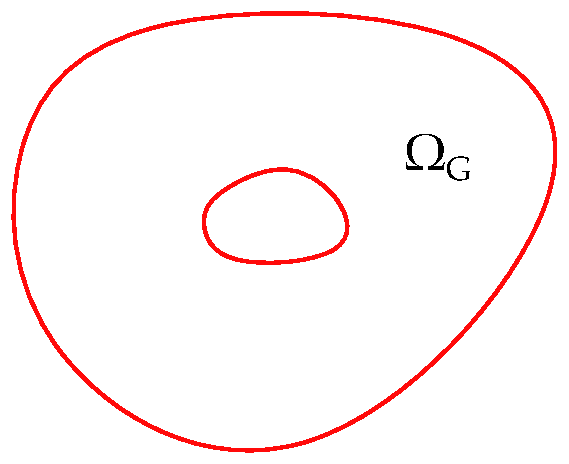
\includegraphics[scale=0.6,trim=0cm 0cm 0cm 0cm, clip=true]{Imagens/Cap5/dominio_global.pdf}} 
	\subfloat[\label{fig:dominio_local} Domínio Local]{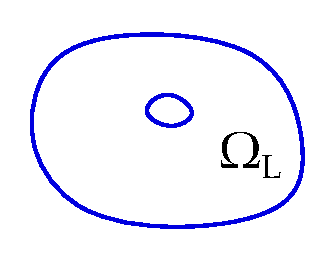
\includegraphics[scale=0.6,trim=0cm 0cm 0cm 0cm, clip=true]{Imagens/Cap5/dominio_local.pdf}} \\
	\subfloat[\label{fig:dominio_sobreposto} Domínios sobrepostos]{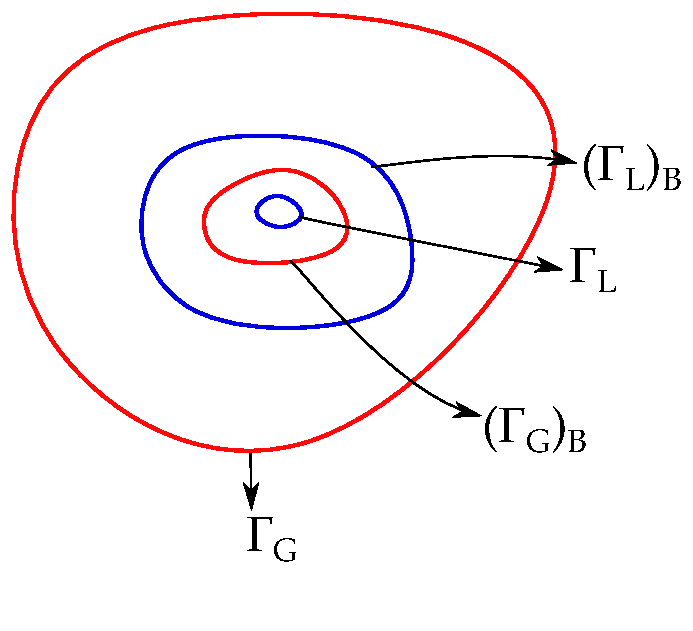
\includegraphics[scale=0.6,trim=0cm 0cm 0cm 0cm, clip=true]{Imagens/Cap5/dominio_sobreposto.pdf}} 
	\label{fig:domains}
	\legend{Fonte: Elaborada pela autora}
\end{figure}

Considerando um problema cujas funções tentativa nos domínios global e local seja caracterizada respectivamente por $u_{G}(\pos)$, definida no espaço finito de funções $\usolution^{G}$, e  $u_{L}(\pos)$, definida no espaço finito de funções $\usolution^{L}$, sendo as funções teste global $w_{G}(\pos)$ e local $w_{L}(\pos)$ definidas nos espaços $\uweighting^{G}$ e $\uweighting^{L}$, respectivamente. A união direta dos espaços de funções na zona de sobreposição obviamente não resulta em um espaço que respeita a partição da unidade nas funções de forma e nem que seja garantida a independência linear. 
Dessa forma, utiliza-se uma função ponderadora de combinação $b(\pos)$, de maneira que as funções tentativa e teste sejam:

\begin{align}
u(\pos) = b(\pos)u_{G}(\pos) + (1-b(\pos))u_{L}(\pos),\\
w(\pos) = b(\pos)w_{G}(\pos) + (1-b(\pos))w_{L}(\pos),
\end{align}

\noindent com $b(\pos)$ apresentando valor unitário sobre o domínio global livre (sem sobreposições), valor zero no domínio local livre, e apresentando uma transição suave na região de sobreposição. 

Os espaços enriquecidos na região de superposição de malhas, são definidos por $\mathcal{S}_{enr}$ e $\mathcal{V}_{enr}$, correspondentes às funções tentativa e teste respectivamente. A solução de um problema típico de valor de contorno recai em encontrar $u^{h} \in \mathcal{S}_{enr}$ tal que $\forall$ $ w^{h} \in \mathcal{V}_{enr}$: 

\begin{align}
B(u^{h},w^{h}) = F(w^{h}),
\end{align}

\noindent com $B(\bullet,\bullet)$ e $F(\bullet)$ sendo operadores bilineares e lineares respectivamente. A discretização de $u^{h}(\pos)$ e $w^{h}(\pos)$ no contexto dos elementos finitos é obtida através das seguintes relações:

\begin{align}
u^{h}(\pos) = \sum_{A = 1}^{(n_{np})_G} (u_{G})_{A}b(\pos)(N_{G})_{A}(\pos) + \sum_{A = 1}^{(n_{np})_L} (u_{L})_{A}(1-b(\pos))(N_{L})_{A}(\pos),\label{eq:u_mod} \\ 
w^{h}(\pos) = \sum_{A = 1}^{(n_{np})_G} (w_{G})_{A}b(\pos)(N_{G})_{A}(\pos) + \sum_{A = 1}^{(n_{np})_L} (w_{L})_{A}(1-b(\pos))(N_{L})_{A}(\pos), \label{eq:w_mod}
\end{align}

\noindent com $N_{G}$ e $N_{L}$ sendo as funções de forma global e local; e $(n_{np})_G$ e $(n_{np})_L$ o número de funções de forma nas discretizações global e local respectivamente. 

\section{Função de combinação}

Considerando que as funções $b(\pos)(N_{G})$ e $(1-b(\pos))(N_{L})$ sejam linearmente independentes sobre $\Omega_{B}$, e que as funções base local e global sejam discretizadas com polinômios de igual ordem $p$ e constituam funções base independentes dentro das discretizações local e global, a escolha de $b$ um grau acima das funções base, ou seja, grau $p+1$, irá proporcionar uma nova base de grau consistente com o número de funções base disponíveis em cada ponto da zona de superposição. A nova base, que continua sendo um polinômio de grau $p$ fora do domínio de sobreposição, torna-se um polinômio de ordem $2p+1$ dentro da zona de sobreposição, evitando dependência linear entre as funções de forma e cumprindo a partição da unidade.

Nesse trabalho aplicam-se funções de forma locais e globais de grau polinomial quadrático. Dessa forma, a função ponderadora de combinação foi definida como cúbica e é expressa por:

\begin{align}
b(\pos) =  \begin{cases} 2\left(\frac{Y_{L}(\pos)}{\delta(\pos)}\right)^3  -   3\left(\frac{Y_{L}(\pos)}{\delta(\pos)}\right)^2   \mbox{se } Y_{G}(\pos)> 0 \ e \ Y_{L}(\pos)> 0 \\
1  \ Y_{L}(\pos) \leq 0  \\
0  \ Y_{G}(\pos) \leq 0 \end{cases},
\end{align}

\noindent com $Y_{L}(\pos)$ a função distância assinalada medida a partir de $(\Gamma_{L})_{B}$, com valores positivos dentro do domínio local e negativos fora, e $Y_{G}(\pos)$ a função distância assinalada medida a partir de $(\Gamma_{G})_{B}$, sendo positiva se o ponto pertence à $\Omega_{G}$, e negativa, caso contrário. Nota-se que os pontos em que ambas funções distância assinalada são positivas estão contidos dentro da zona de sobreposição. O parâmetro $\delta$ é obtido por $\delta(\pos) = Y_{L}(\pos) + Y_{G}(\pos)$, e coincide com a espessura da zona de sobreposição quando $(\Gamma_{L})_{B}$ e $(\Gamma_{G})_{B}$ são paralelos.

Na prática, considera-se que o domínio global tem o tamanho do domínio total, ficando a definição de $(\Gamma_{G})_{B}$ para uma etapa posterior, baseado na forma do modelo local. Os elementos e nós da malha global, sem suporte físico após a obtenção do novo espaço de funções, são desativados da análise. O contorno $(\Gamma_{G})_{B}$ pode ser obtido através de uma réplica do contorno $(\Gamma_{L})_{B}$ a uma distância paralela $\delta$ do mesmo. 

Após a definição $(\Gamma_{G})_{B}$ é necessária uma metodologia eficiente para determinação das funções base globais com pequena influência dentro da zona de sobreposição, visto que essas podem levar a um sistema mal condicionado. Para resolver esse problema, utiliza-se, para todos os nós globais A da análise, uma variável definida como:

\begin{align}
	(M_{G})_{AA} = \int_{\Omega}b(\bm{\xi})N_{A}(\bm{\xi})b(\bm{\xi})N_{A}(\bm{\xi})d\Omega, \label{eq:influence}
\end{align}

\noindent e define-se um valor $M_{min}$ para $(M_{G})_{AA}$. Os nós globais são desativados se $(M_{G})_{AA} < M_{min}$. 

Na Figura \ref{fig:funcoes_tecnica_particao} apresenta-se um exemplo unidimensional da técnica de partição de domínios. Na Figura \ref{fig:funcoes_dominio_global} observam-se as funções globais definidas inicialmente sobre todo o domínio, e a função ponderadora de modificação $b(y)$ com valor unitário sobre o domínio global livre e com transição suave sobre a região de sobreposição. Na Figura \ref{fig:funcoes_dominio_local} representam-se as funções locais definidas somente no domínio local e a função ponderadora de modificação $1-b(y)$ com valor unitário sobre o domínio local livre e com transição suave sobre a zona de sobreposição. Por fim, na Figura \ref{fig:funcoes_modificadas} apresenta-se o novo espaço de funções independentes que cumprem com a partição da unidade e possuem grau polinomial $5$. Nota-se nessa figura a desativação das funções de forma globais que estão sobre o domínio local livre.

\begin{figure}[!htbp]
	\caption{Espaços de funções na técnica de partição de domínios - Problema unidimensional}
	\centering
	\subfloat[\label{fig:funcoes_dominio_global} Funções globais e função ponderadora ($b$).]{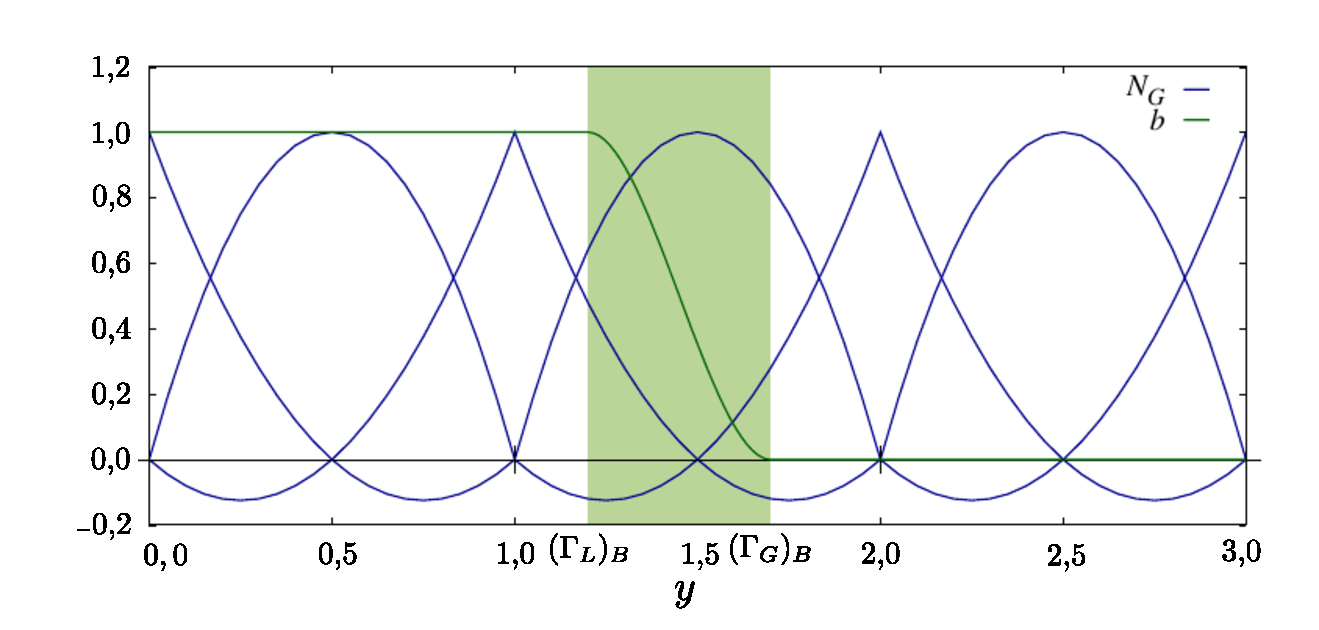
\includegraphics[scale=0.6, trim=0cm 0cm 0cm 0cm, clip=true]{Imagens/Cap5/funcoes_dom_global.pdf}} \\
	\subfloat[\label{fig:funcoes_dominio_local} Funções locais e função ponderadora ($1-b$) ]{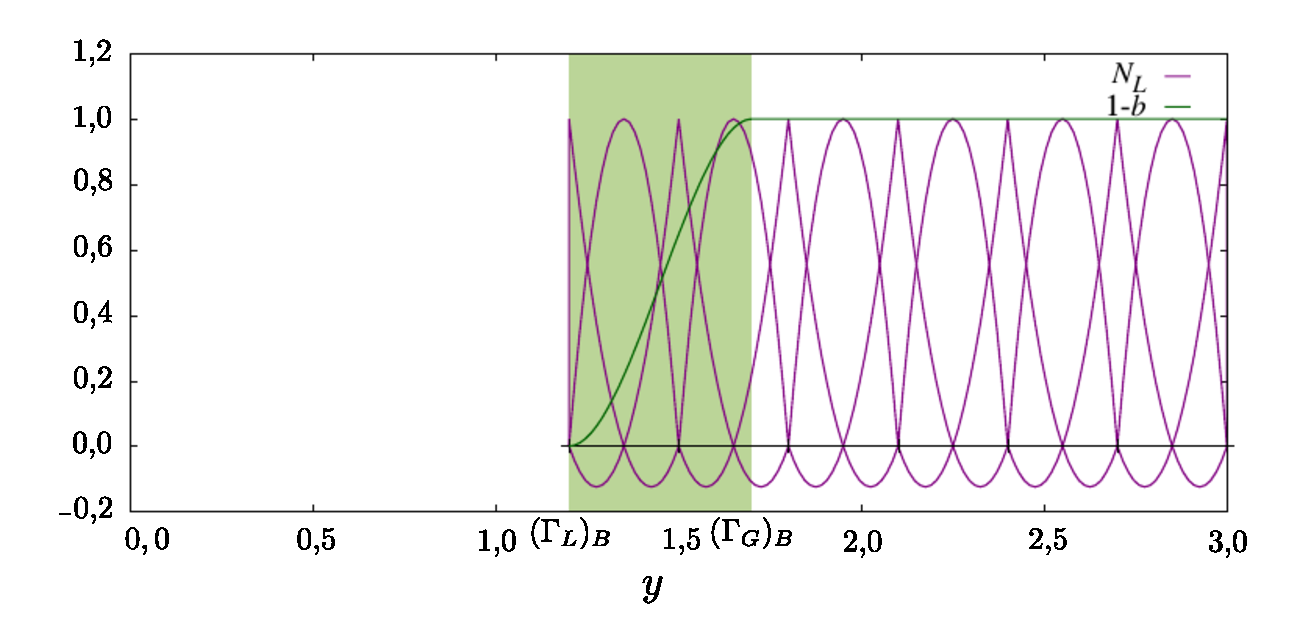
\includegraphics[scale=0.6,trim=0cm 0cm 0cm 0cm, clip=true]{Imagens/Cap5/funcoes_dom_local.pdf}} \\
	\subfloat[\label{fig:funcoes_modificadas} Novo espaço de funções]{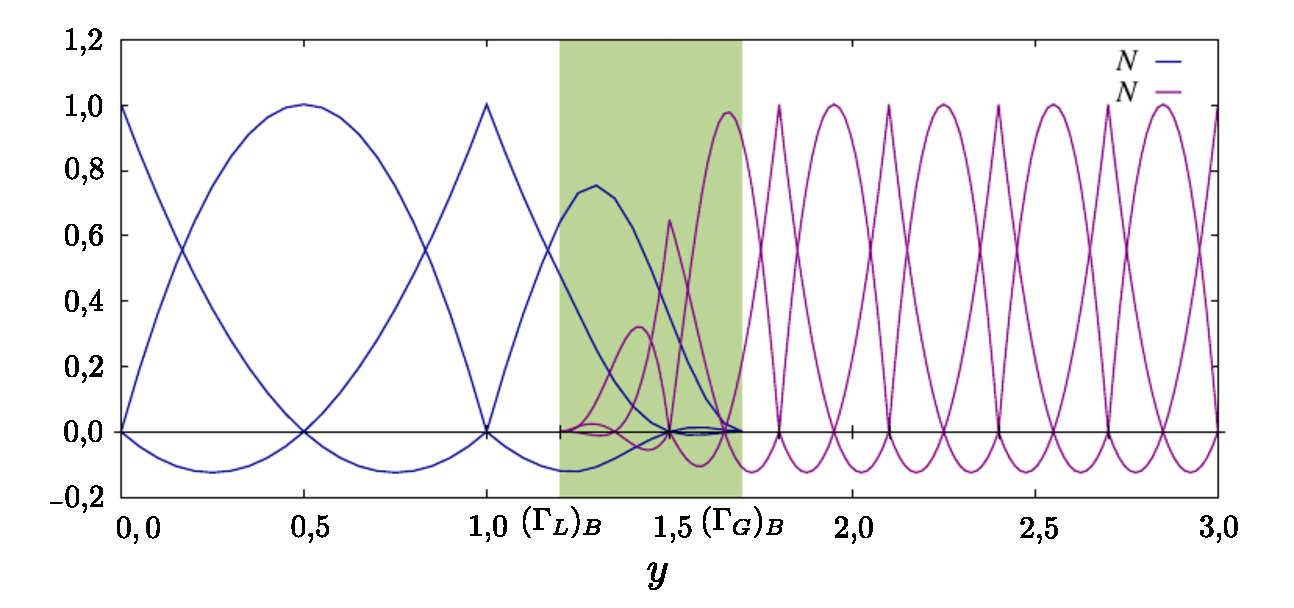
\includegraphics[scale=0.6,trim=0cm 0cm 0cm 0cm, clip=true]{Imagens/Cap5/funcoes_modificadas.pdf}} 
	\label{fig:funcoes_tecnica_particao}
	\legend{Fonte: Elaborada pela autora}
\end{figure}

\section{Aplicação da técnica a Dinâmica dos Fluidos Computacional}

Para o emprego da metodologia nas análises da DFC as aproximações apresentadas nas \autoref{eq:u_mod} e \autoref{eq:w_mod} devem ser aplicadas nas funções tentativa para velocidade e pressão, e nas funções teste associadas à elas, apresentadas nas \autoref{eq:interp_vel} à \autoref{eq:inter_ptest}.

Conforme relatado, os parâmetros de estabilização utilizados na técnica da DFC ainda necessitam de um estudo mais aprofundado, entretanto, para estudos iniciais, fez-se a combinação dos parâmetros calculados em cada uma das discretizações sobre a zona de sobreposição:

\begin{align}
\SUPG(\pos) =  b(\pos)(\SUPG)^{G}(\pos) + (1-b(\pos))(\SUPG)^{L}(\pos),\\
\PSPG(\pos) =  b(\pos)(\PSPG)^{G}(\pos) + (1-b(\pos))(\PSPG)^{L}(\pos),\\
\LSIC(\pos) =  b(\pos)(\LSIC)^{G}(\pos) + (1-b(\pos))(\LSIC)^{L}(\pos),
\end{align}

\noindent com $(\SUPG)^{G}$, $(\PSPG)^{G}$ e $(\LSIC)^{G}$ os parâmetros de estabilização calculados na malha global;$(\SUPG)^{L}$, $(\PSPG)^{L}$ e  $(\LSIC)^{L}$ os parâmetros de estabilização calculados na malha local, todos conforme a Eq. \textcolor{red}{Colocar referência para a eq que define os parâmetros}.

\section{Implementação Computacional}

O método dos espaços de funções combinados foi implementado para a solução de escoamentos incompressíveis seguindo a formulação apresentada nos capítulos \ref{capitulo:Cap2} e \ref{capitulo:Cap3}. Nesse código, após a leitura dos dados respectivos às malhas global e local, segue-se com a definição da distância assinalada respectiva a todos os nós da malha global e da malha local com respeito aos contornos $(\Gamma_{G})_{B}$ e $(\Gamma_{L})_{B}$, respectivamente. O contorno  $(\Gamma_{G})_{B}$ é obtido a partir dos dados de entrada, onde define-se a espessura da zona de sobreposição. De posse da distância assinalada e espessura da zona de sobreposição, são definidos quais elementos das malhas local e global fazem parte da zona de sobreposição. Qualquer elemento que possua 1 ou mais nós dentro da zona de sobreposição é considerado como um elemento contribui com ela.

As equações na região de sobreposição são integradas sobre o elemento local, dessa forma, no pré-processamento, os pontos de integração da malha local são projetados sobre a malha global e o elemento global e suas coordenadas paramétricas correspondentes a cada ponto são armazenados. 

Na etapa de pré-processamento, são determinados ainda os nós inativos da malha global, sejam porque o domínio de suas funções de forma encontram-se fora da zona de sobreposição, ou, porque possuem pequena influência dentro da mesma, de acordo com a expressão apresentada na \autoref{eq:influence}.

Finalmente, o processo de marcha no tempo se inicia da maneira explicitada no Item \ref{capitulo:Cap2:DFCComputationalCode} levando-se em consideração que as funções tentativa e peso, e os parâmetros de estabilização são modificados de acordo com o apresentado neste capítulo. O algoritmo que descreve esse processo de solução pode ser visualizado no Alg. \ref{alg:overlap}.

\begin{algorithm}
	\caption{Algoritmo para problemas da dinâmica dos fluidos computacional com a técnica de partição de domínios}
	\label{alg:overlap}
	\begin{algorithmic}[1]
		\State Cálculo da distância assinalada dos nós e pontos de controle aos contornos;
		\State Determinação dos elementos e células da zona de sobreposição;
		\State Busca da correspondência dos pontos de integração da malha local na malha global;
		\State Definição dos nós inativos da malha global;
		\For {o passo de tempo $0$ até $\totalTime$} 
		\State $i=0$;
		\State Predição da solução: aplicação das \autoref{eq:pred_acel}, \autoref{eq:pred_vel} e \autoref{eq:pred_press};
		\While{($\epsilon$ < tolerância)}
		\State $i$++;
		\State Interpolação das variáveis do problema: aplicação da \autoref{eq:inter_acel_i}, \autoref {eq:inter_vel_i} e \autoref{eq:inter_press_i};
		\State Cálculo do incremento nas variáveis do problema: $\Acceleration_{n+1}$ e $\Press_{n+1}$ de acordo com as \autoref{eq:eq_lin_QM} e \autoref{eq:eq_lin_cont};
		\State Atualização da solução: calculadas de acordo com \autoref{atu_acel}, \autoref{atu_vel} e \autoref{atu_press}.
		\State Cálculo do erro:
		\begin{align}
			\epsilon =\left\| \NNSM^i \right\|_{L^2}
		\end{align}
		\EndWhile
		\State Atualização das variáveis do passo anterior;
		\EndFor
	\end{algorithmic}
\end{algorithm}

\section{Exemplo - Cavidade com partição de domínio e combinação MEF-IGA} \label{capitulo:cap5:Exemplo}

Para verificar a metodologia de partição de domínios com sobreposição de malhas, neste item apresenta-se a solução estacionária do problema de Navier Stokes para a cavidade 2D.

A geometria do problema e suas condições contorno são apresentadas na \autoref{fig:cav2d_geometria}. O problema foi avaliado para um número de Reynolds = 100, calculado de acordo com \autoref{eq:Reynolds} e $\rho = 1,0$.

\begin{figure}[!htbp]
	\caption{Cavidade: geometria e condições de contorno} 
	\centering
	{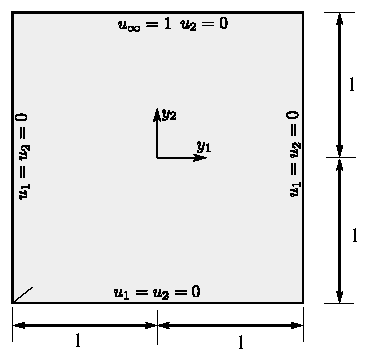
\includegraphics[scale=1.3,trim=0cm 0cm 0cm 0cm, clip=true]{Imagens/Cap5/cav2d_geometria.pdf}}
	\label{fig:cav2d_geometria}
	\legend{Fonte: Elaborada pela autora}
\end{figure}

Sabe-se que nas paredes da cavidade podem haver efeitos de camada limite, dessa forma, definiu-se uma malha local que circunda a cavidade de acordo com a Figura \ref{fig:cav2d_malha_local}. A malha local foi discretizada através de uma aproximação isogeométrica e foi definida com 1440 pontos de controle que foram divididos em 8 diferentes \textit{patches}, chamados de $P_{1},P_{2},...,P_{8}$. Os \textit{patches} $P_{1},P_{3},P_{6}$ e $P_{6}$ possuem 64 células e os $P_{2},P_{4},P_{5}$ e $P_{7}$ 192 células.

A malha global por sua vez é definida para toda a seção da cavidade, sendo composta por 800 elementos triangulares quadráticos e 1681 nós, de acordo com Figura \ref{fig:cav2d_malha_global}.

\begin{figure}[!htbp]
	\caption{Cavidade 2D: Malhas Global e Local}
	\centering
	\subfloat[\label{fig:cav2d_malha_local} Malha Local]{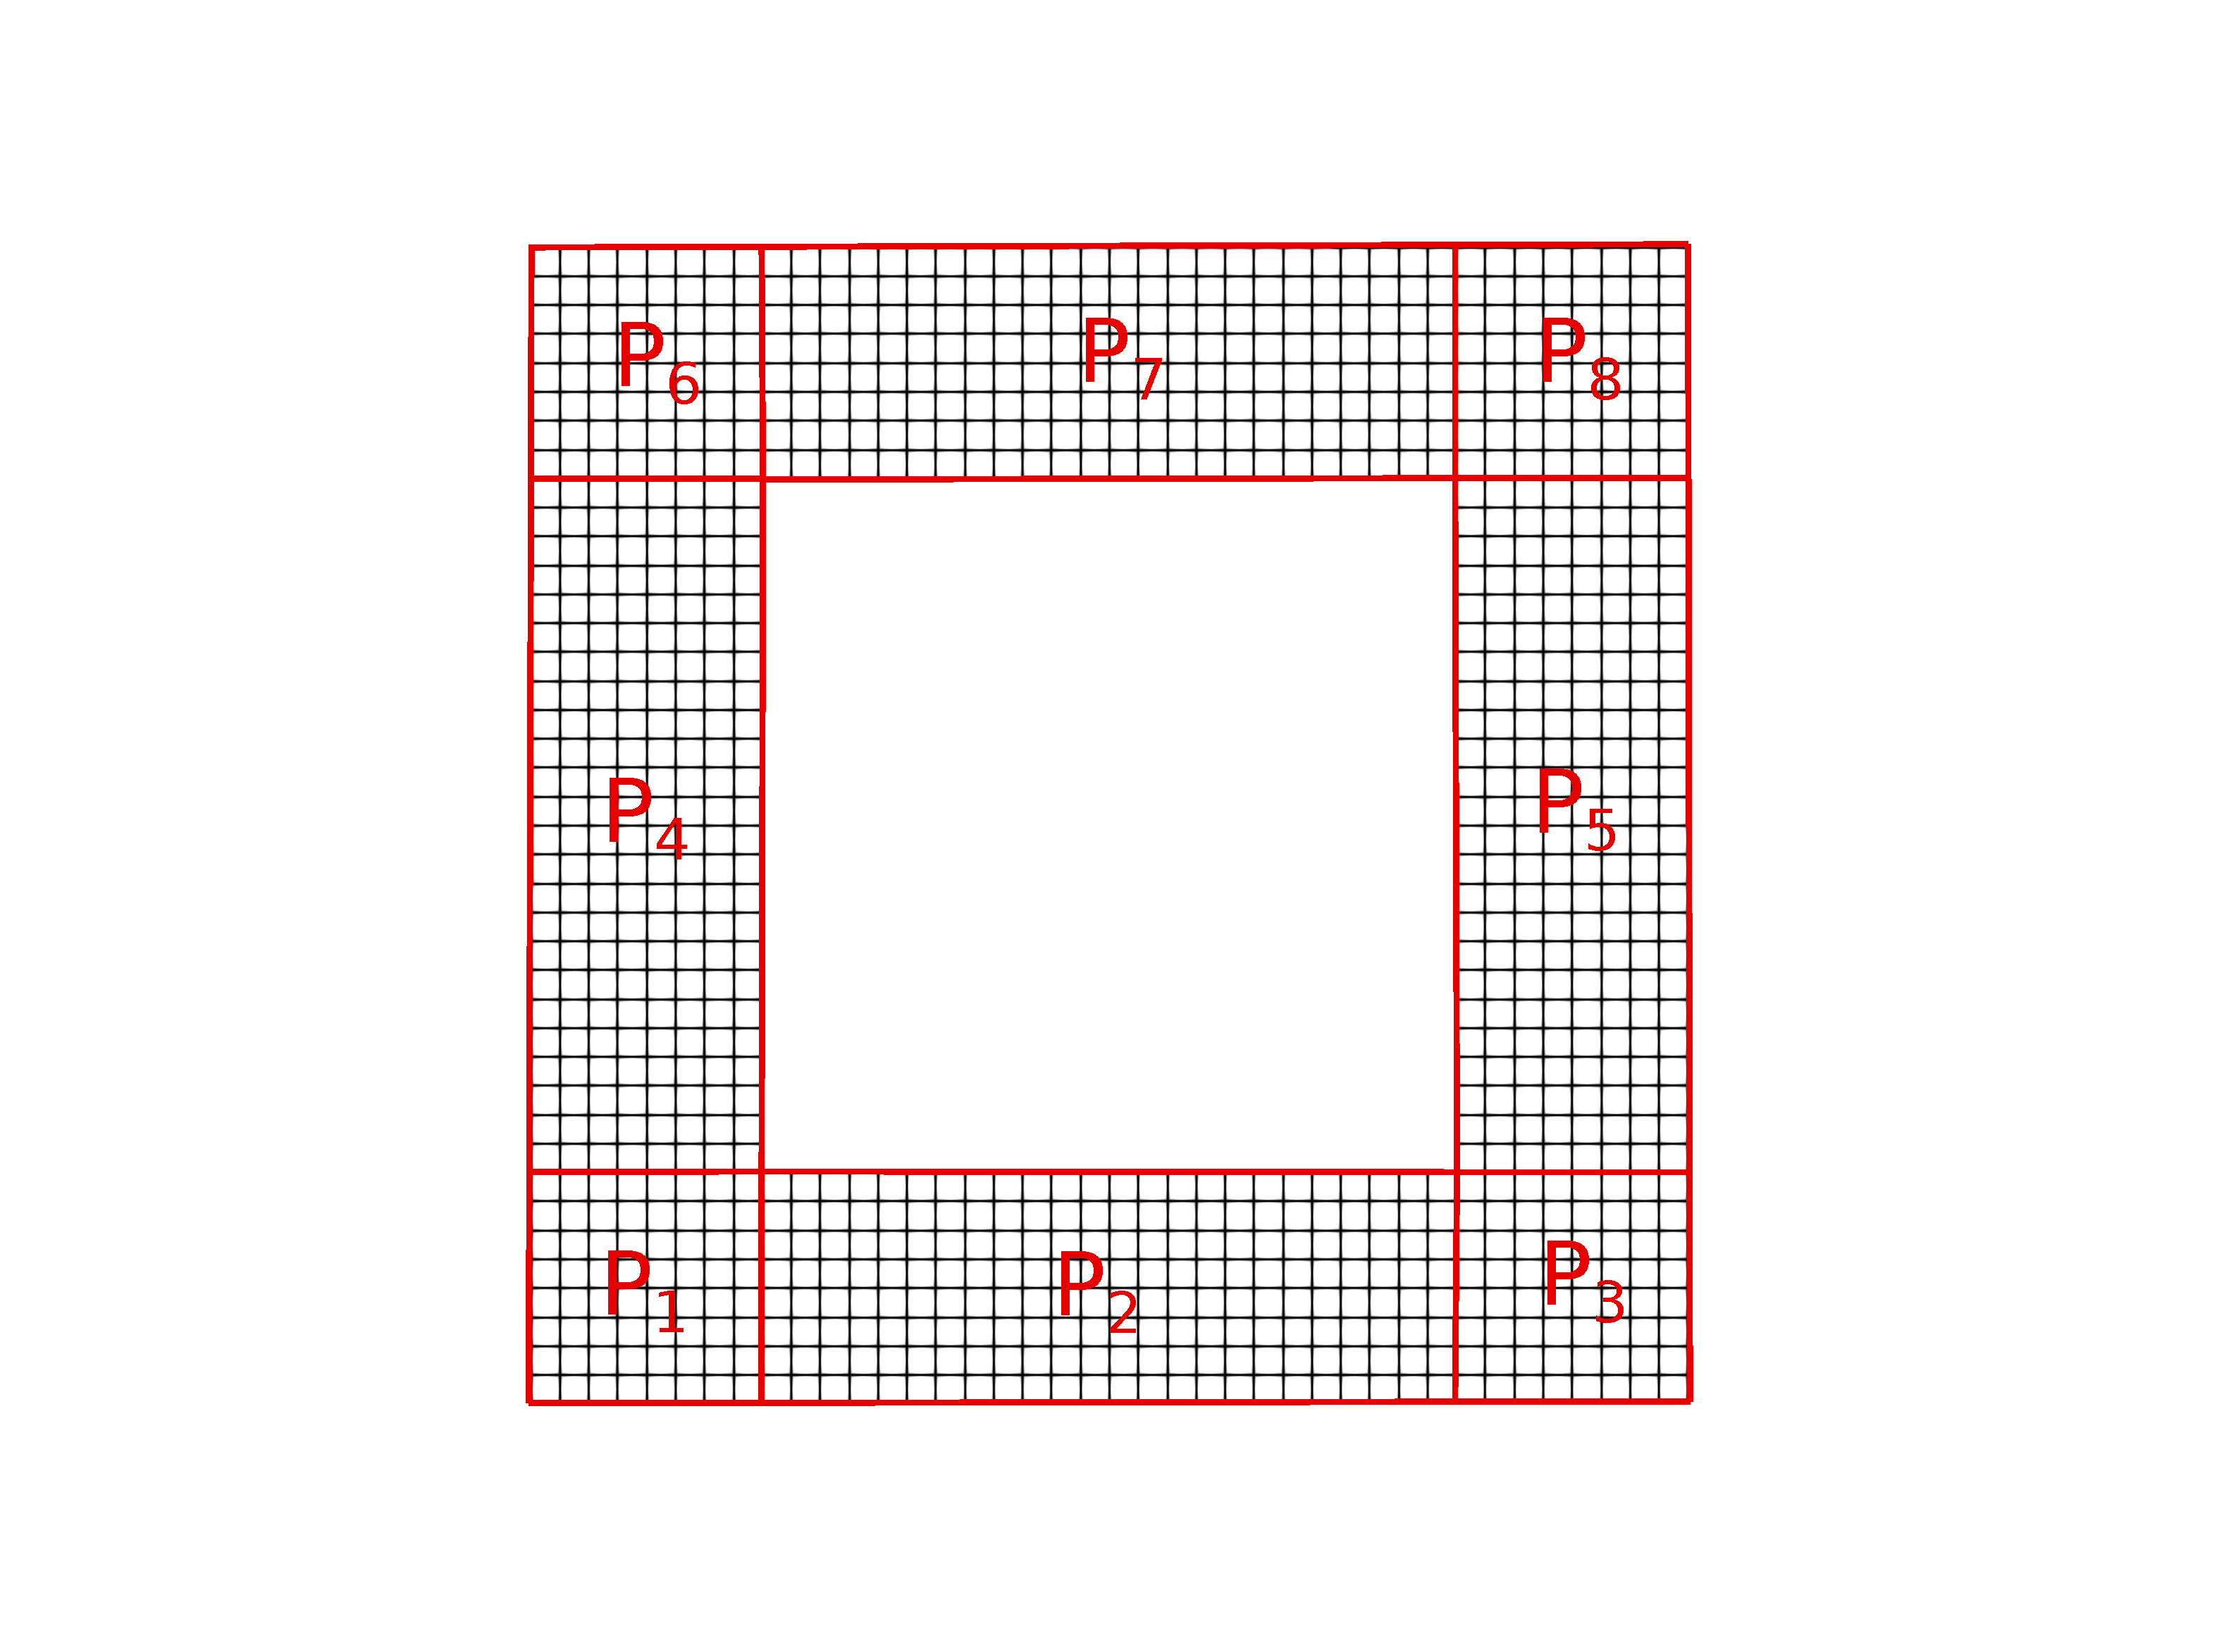
\includegraphics[scale=0.2, trim=9cm 3cm 9cm 5cm, clip=true]{Imagens/Cap5/cav2d_malha_local.pdf}} 
	\subfloat[\label{fig:cav2d_malha_global} Malha Global ]{\includegraphics[scale=0.15,trim=9cm 3cm 9cm 6cm, clip=true]{Imagens/Cap5/cav2d_malha_global.png}}
	\label{fig:cav2d_discretização}
	\legend{Fonte: Elaborada pela autora}
\end{figure}

Definiu-se uma espessura para a zona de sobreposição equivalente a $\delta = 0,1$ e medida paralelamente ao contorno fictício local $(\Gamma_{L})_{B}$. As células e elementos pertencentes à zona de sobreposição, tanto para a malha local quanto para a malha global, podem ser vistos nas Figura \ref{fig:cav2d_elementos_zs_local} e Figura \ref{fig:cav2d_elementos_zs_global}, respectivamente.

\begin{figure}[!htbp]
	\caption{Cavidade 2D: Zona de sobreposição}
	\centering
	\subfloat[\label{fig:cav2d_elementos_zs_local} Malha Local]{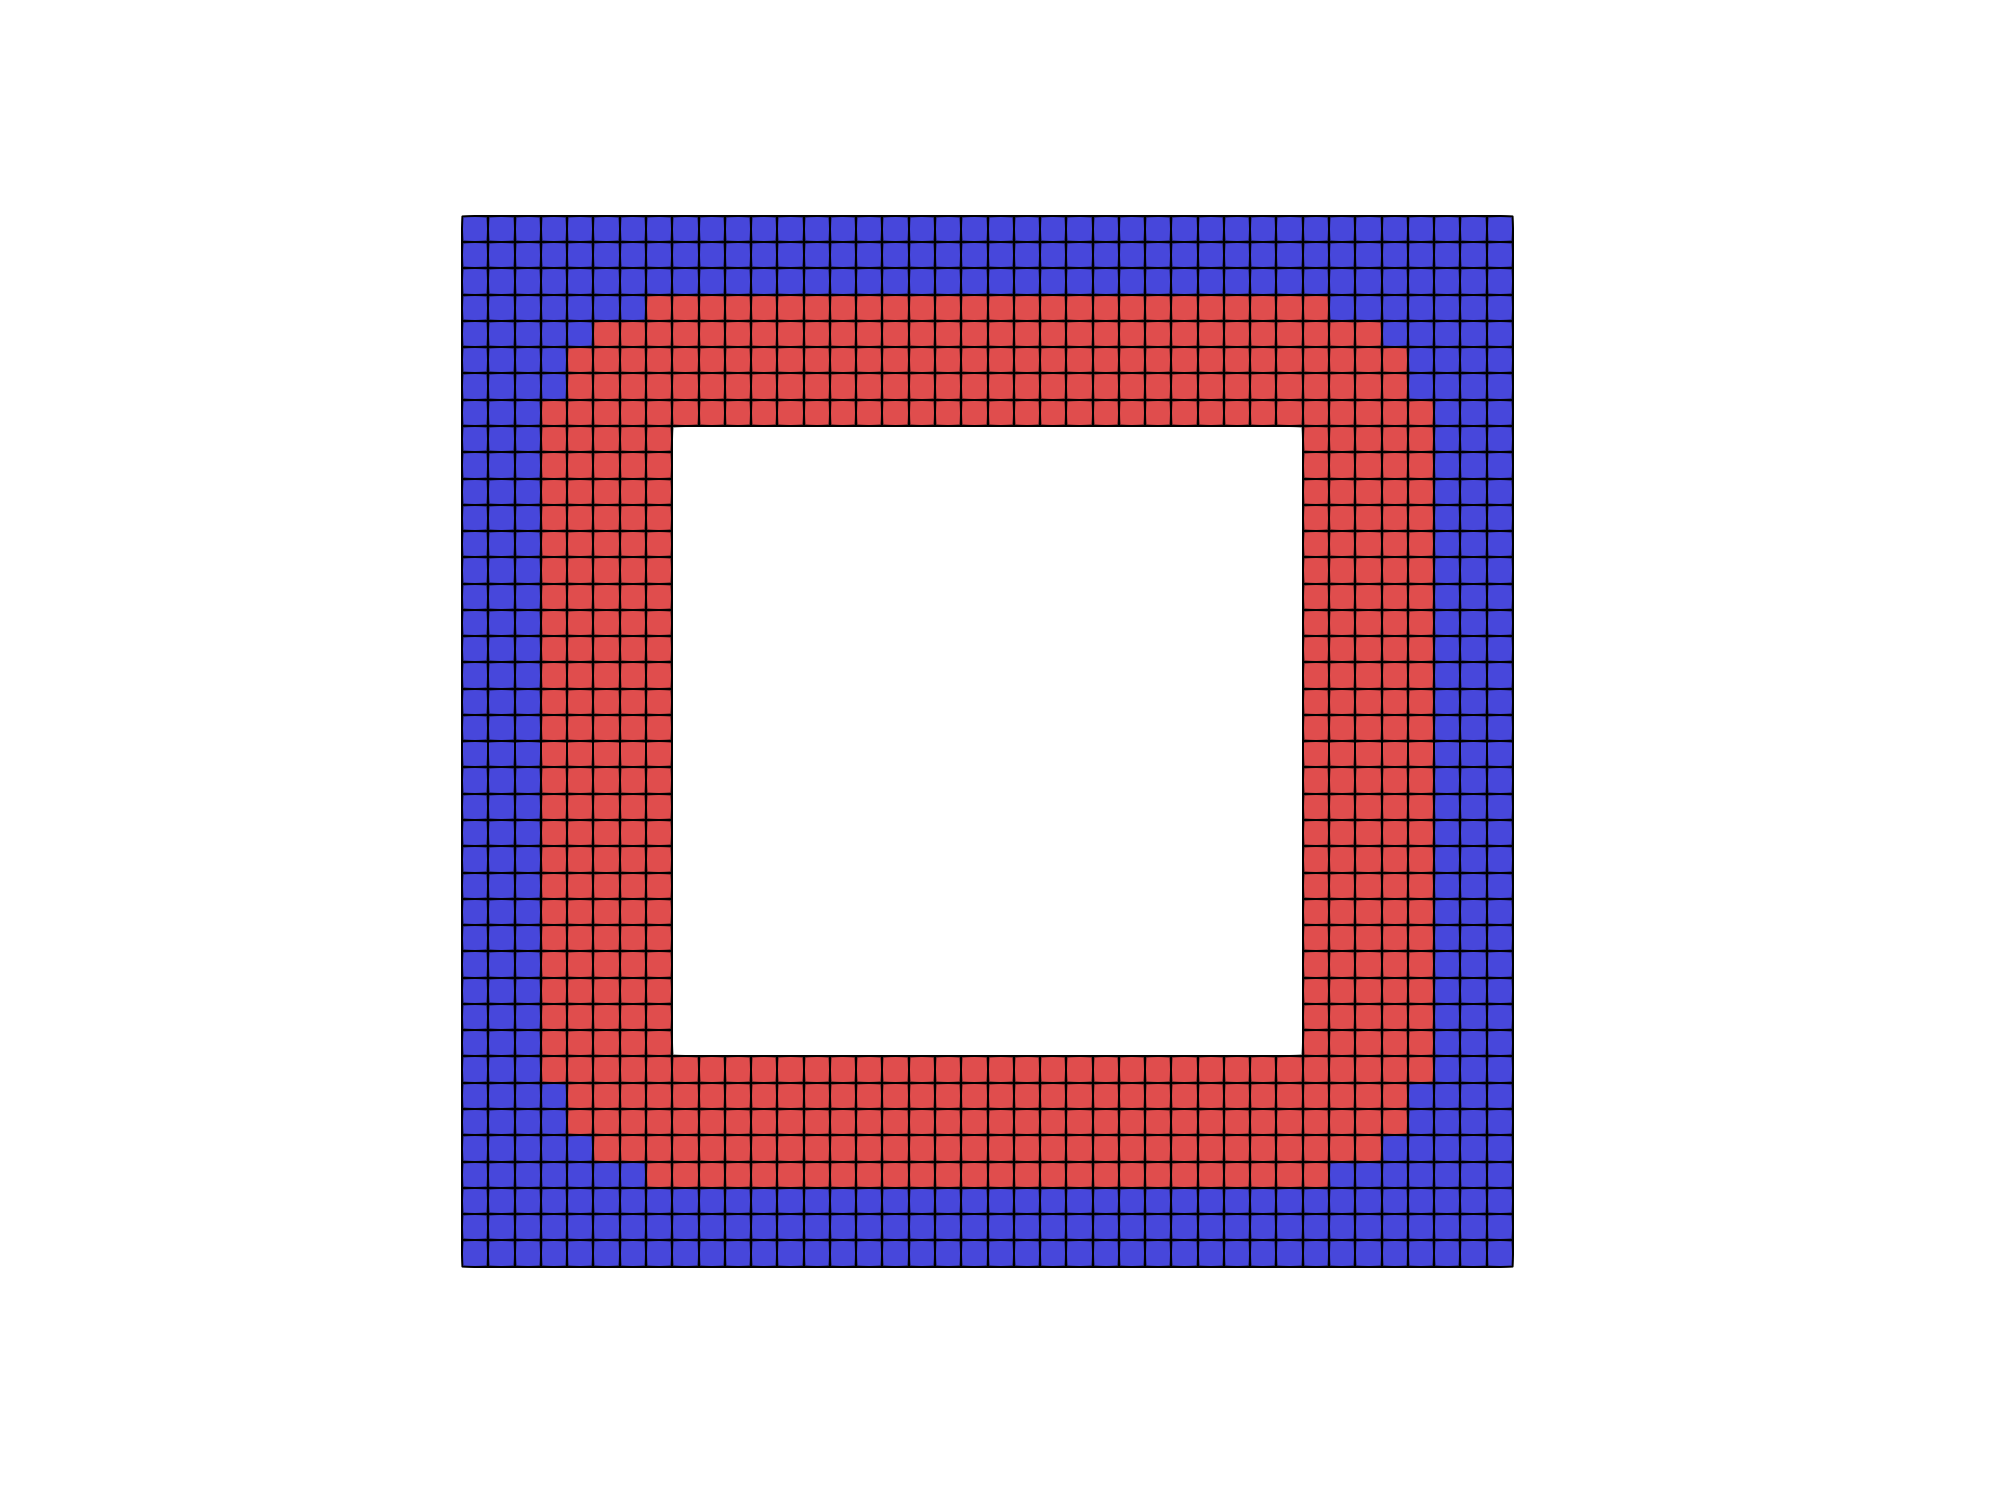
\includegraphics[scale=0.15, trim=10cm 3cm 15cm 6cm, clip=true]{Imagens/Cap5/cav2d_elementos_zs_local.png}} 
	\subfloat[\label{fig:cav2d_elementos_zs_global} Malha Global ]{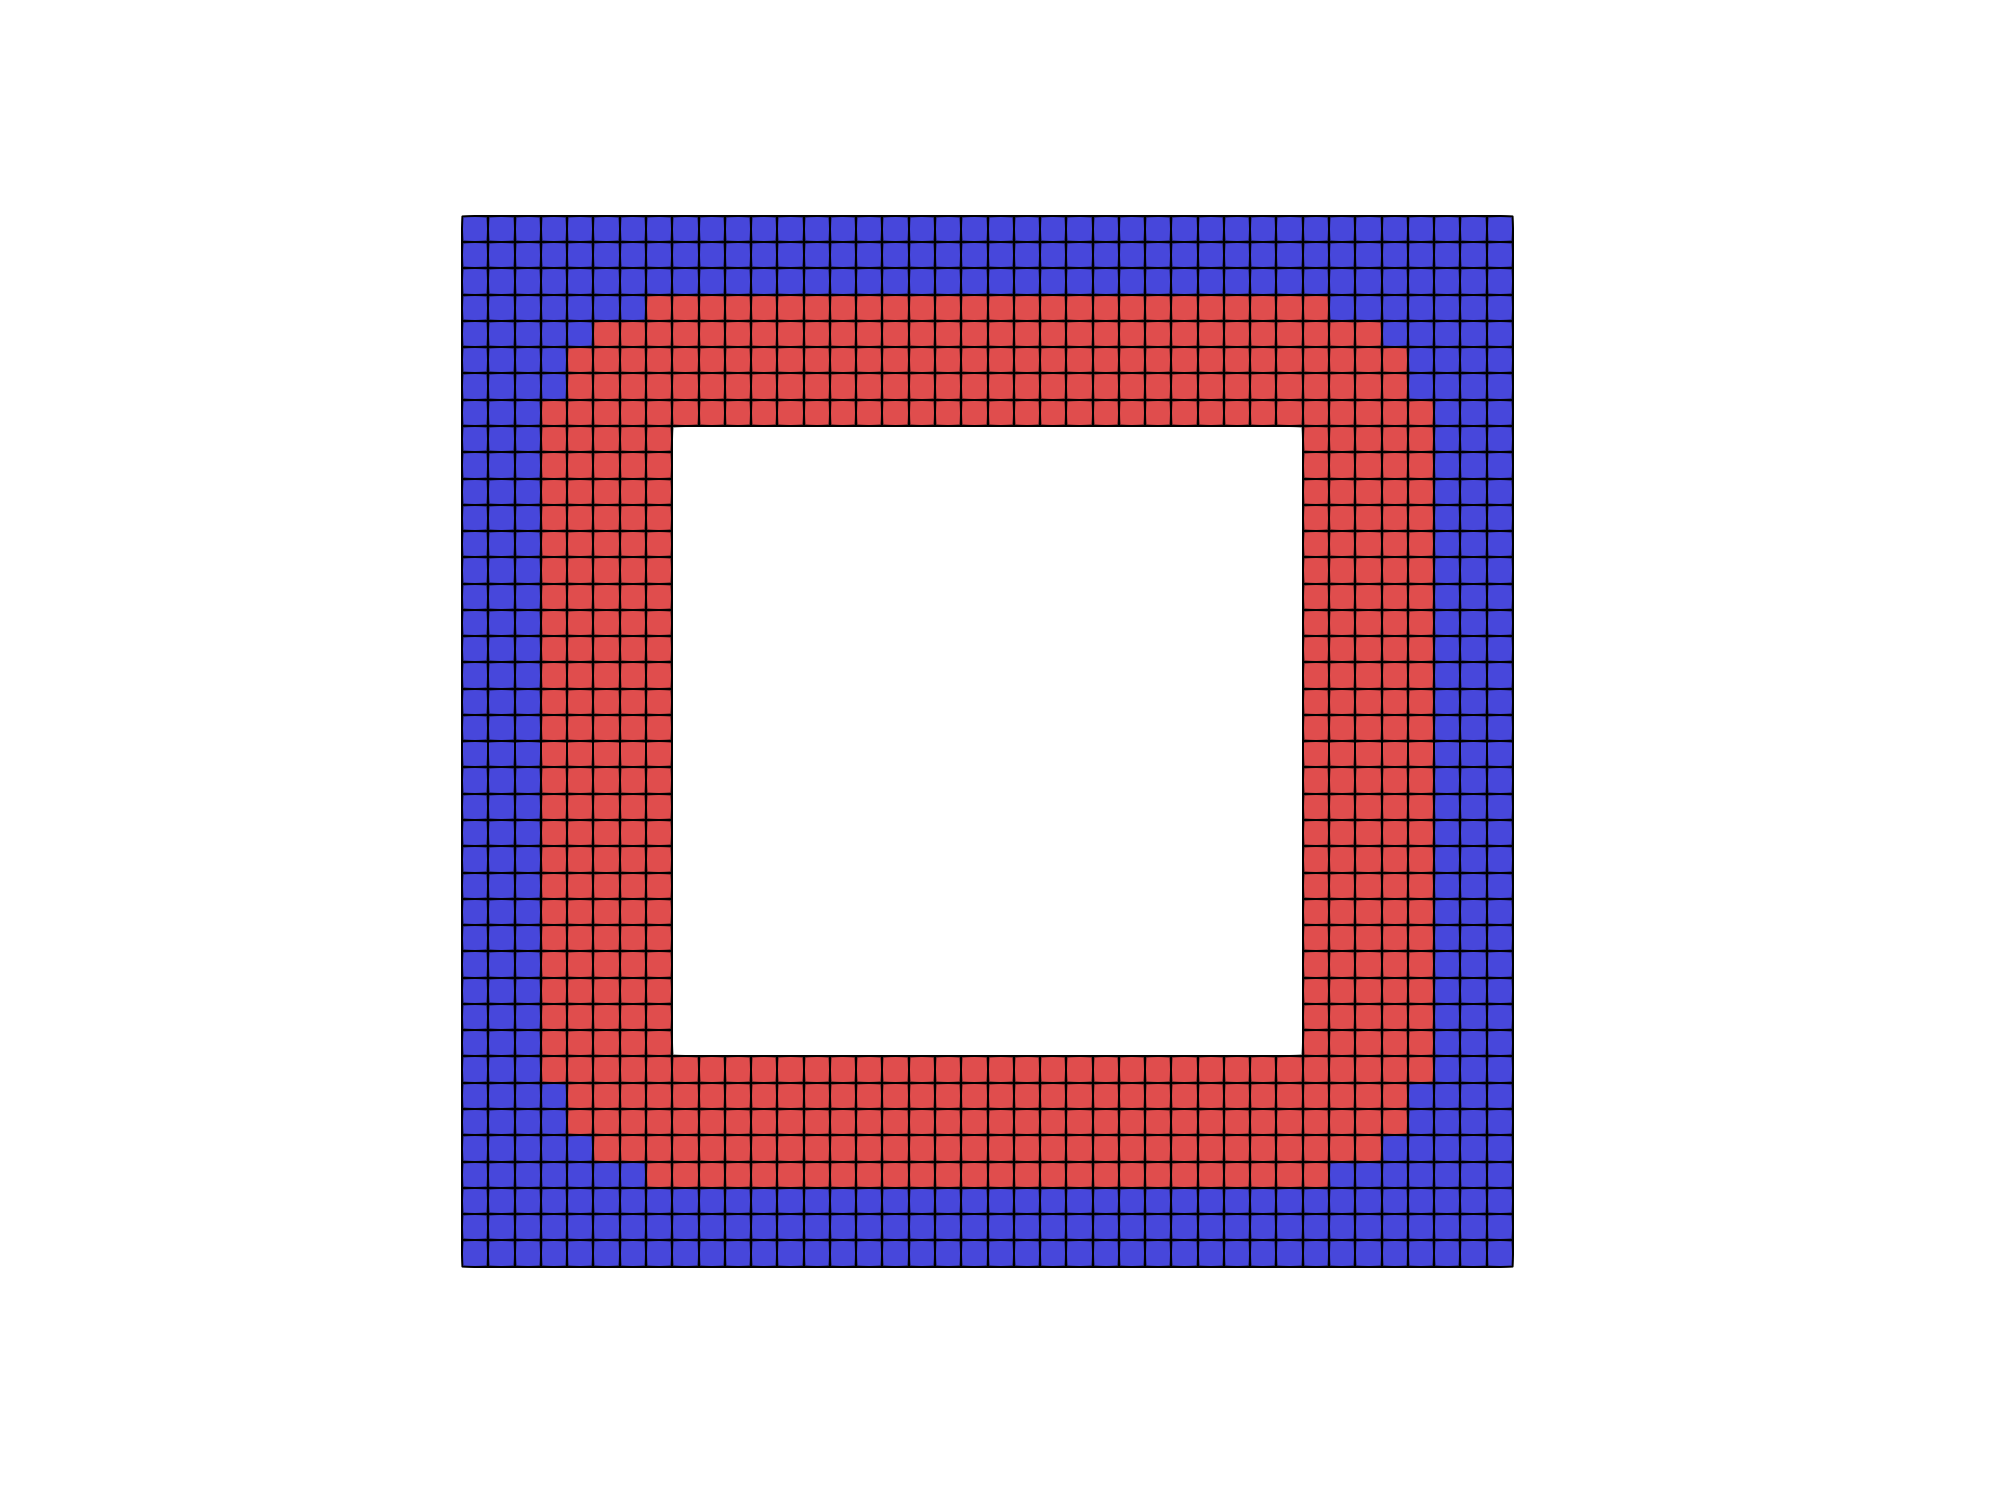
\includegraphics[scale=0.15,trim=10cm 3cm 15cm 6cm, clip=true]{Imagens/Cap5/cav2d_elementos_zs_local.png}}
	\legend{Fonte: Elaborada pela autora}
\end{figure}

Os campos de velocidade e pressão obtidos são apresentados nas Figura \ref{fig:cav2d_campo_velocidade} e Figura \ref{fig:cav2d_campo_pressao}. Os perfis de velocidade adimensionalizados ($\velocity/\velocinfty$) horizontal e vertical ao longo de duas linhas centrais nas direções $y_1$ e $y_2$ da cavidade são apresentados na Figura \ref{fig:cav2d_perfil_vel_Re100} e comparados com os resultados de \citeonline{GhiaGS:1982}.

\begin{figure}[!htbp]
	\caption{Cavidade 2D: Solução do problema de Navier Stokes para $Re = 100$}
	\centering
	\subfloat[\label{fig:cav2d_campo_velocidade} Campo de Velocidade]{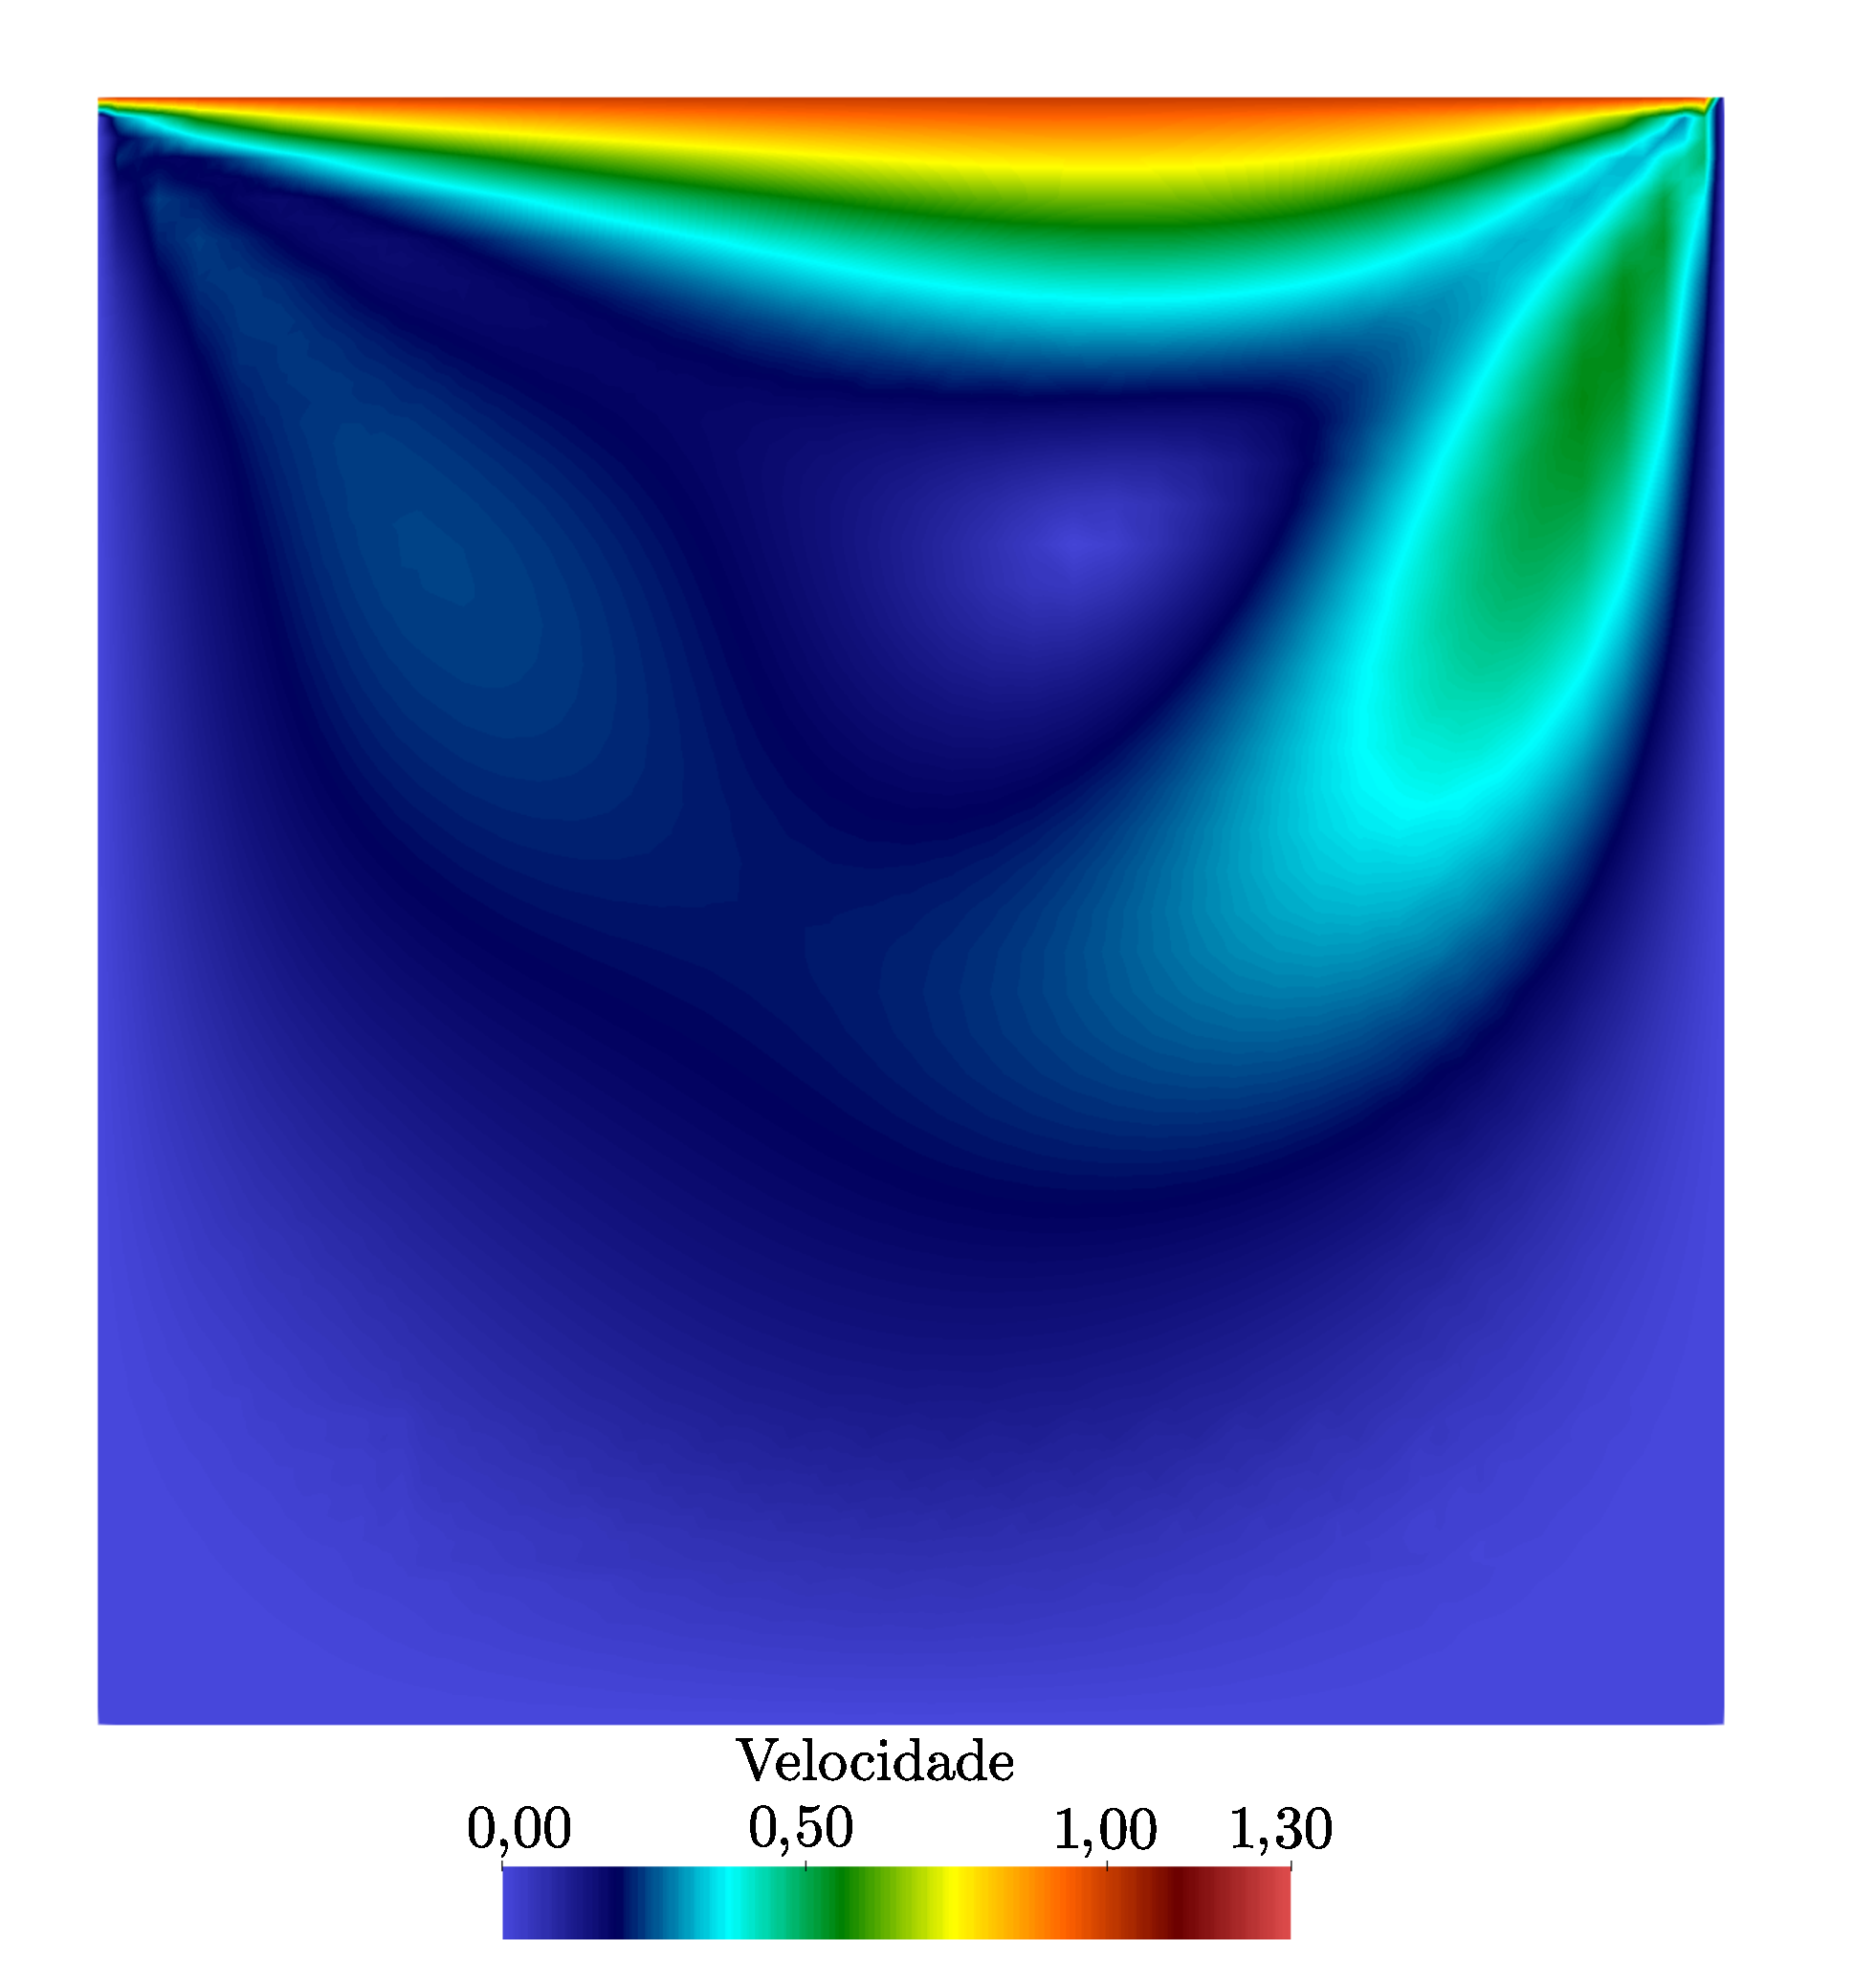
\includegraphics[scale=0.21, trim=0cm 0cm 0cm 0cm, clip=true]{Imagens/Cap5/cav2d_campo_vel.pdf}} 
	\subfloat[\label{fig:cav2d_campo_pressao} Campo de Pressão ]{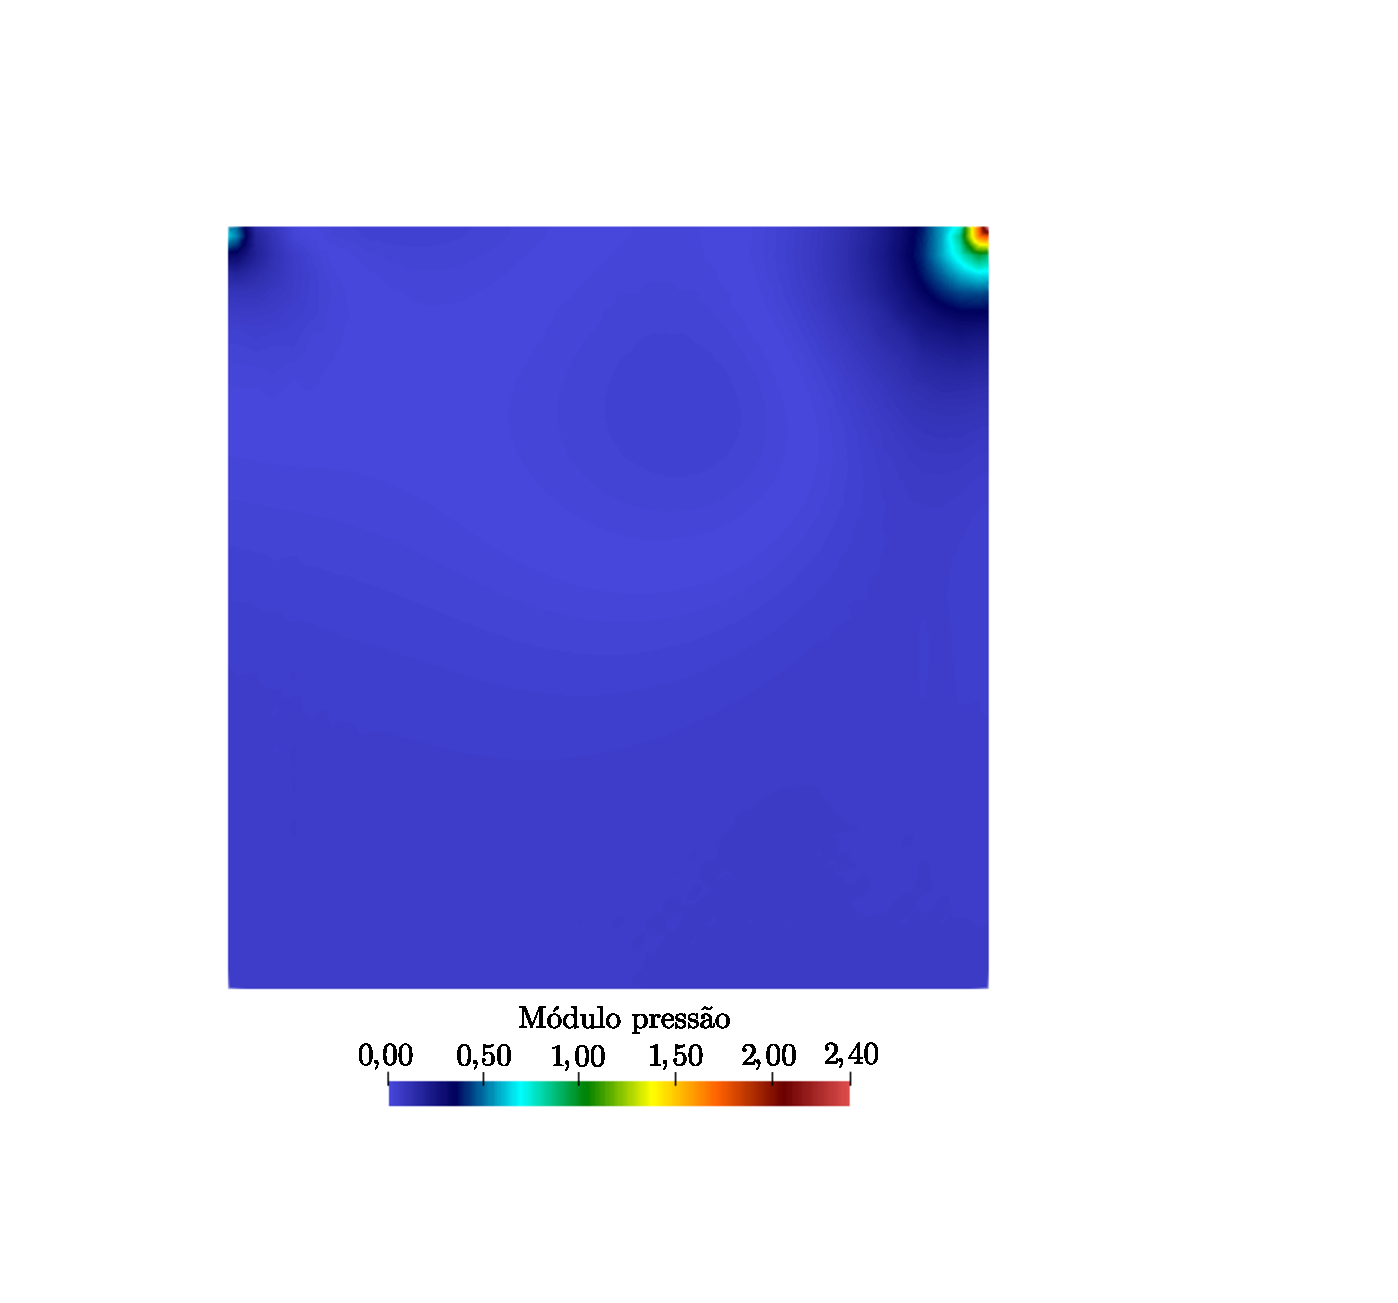
\includegraphics[scale=0.47,trim=3cm 3cm 6cm 3cm, clip=true]{Imagens/Cap5/cav2d_campo_pressao.pdf}}
	\legend{Fonte: Elaborada pela autora}
\end{figure}

\begin{figure}[!!htbp]
	\caption{Cavidade 2D: Perfis de velocidade} 
	\centering
	{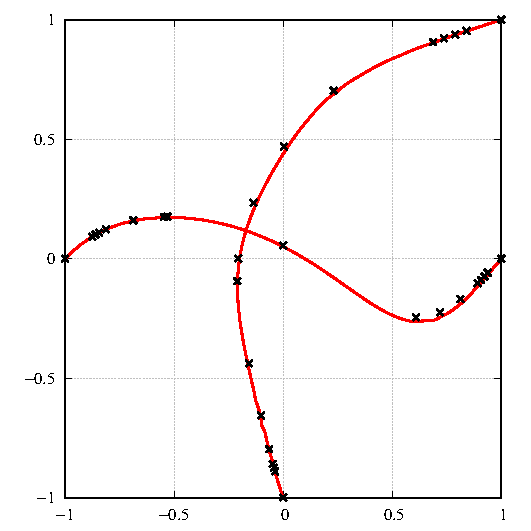
\includegraphics[scale=0.8,trim=0cm 0cm 0cm 0cm, clip=true]{Imagens/Cap5/cav2d_perfil_vel_Re100.pdf}}\\
	{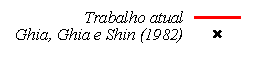
\includegraphics[scale=1.0,trim=0cm 0cm 0cm 0cm, clip=true]{Imagens/Cap5/cav2d_legenda.pdf}}
	\label{fig:cav2d_perfil_vel_Re100}
	\legend{Fonte: Elaborada pela autora}
\end{figure}

\textcolor{red}{Por enquanto vamos deixar assim, mas acho que devemos incluir mais exemplos aqui... Pelo menos exemplos que eu rodei. Na verdade, o importante seria colocar exemplos que apresentaram problema de convergência.}